\section{Cronograma de trabajo}

\subsection{Ciclo de vida}

El ciclo de vida mas pertinente en esta etapa será el modelo en cascada, esto se debe a que el análisis iniciál ya está generado y a su vez los cambios serán entregados de una unica vez al cliente. Se descartaron otros modelos de ciclo de vida al no poseer un equipo muy numeroso y carecer de la habilidad de incluir al cliente en el proceso de desarrollo. \\


\begin{comment}
El ciclo de vida mas pertinente para esta etapa del proyecto es una combinación entre el modelo en cascada y un ciclo iterativo incremental, esto se debe a que si bien las tareas se van a organizar de manera que el proyecto avance generando prototipos usables y estables, es en la fecha final que todos los cambios se van a presentar al cliente. \\
Adems, se irán aplicando incrementalmente, esto es que cada paquete de trabajo concerniente a los cambios a realizar genere un prototipo que sea completamente funcional. \\
Esto nos dá la ventaja de tener un mayor control sobre las tareas de desarrollo restantes.
\end{comment}


\begin{figure}[H]
    \centering
    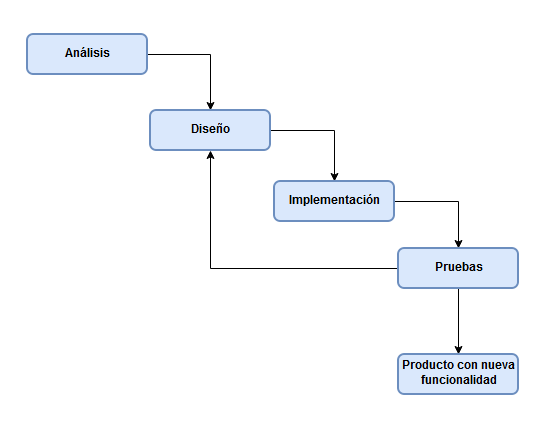
\includegraphics[scale=0.6]{Files/iterativeIncremental.png}
    \caption{Modelo de ciclo de vida}
    \label{fig:clases}
\end{figure}

\subsection{Cronograma}

A continuación se presenta el cronograma de las tareas donde se puede apreciar la forma en que se van a realizar las mismas. Por lo que se puede apreciar las actividades estarán organizadas en el diseño, desarrollo y posterior prueba de las funcionalidades.

\begin{figure}[H]
    \centering
    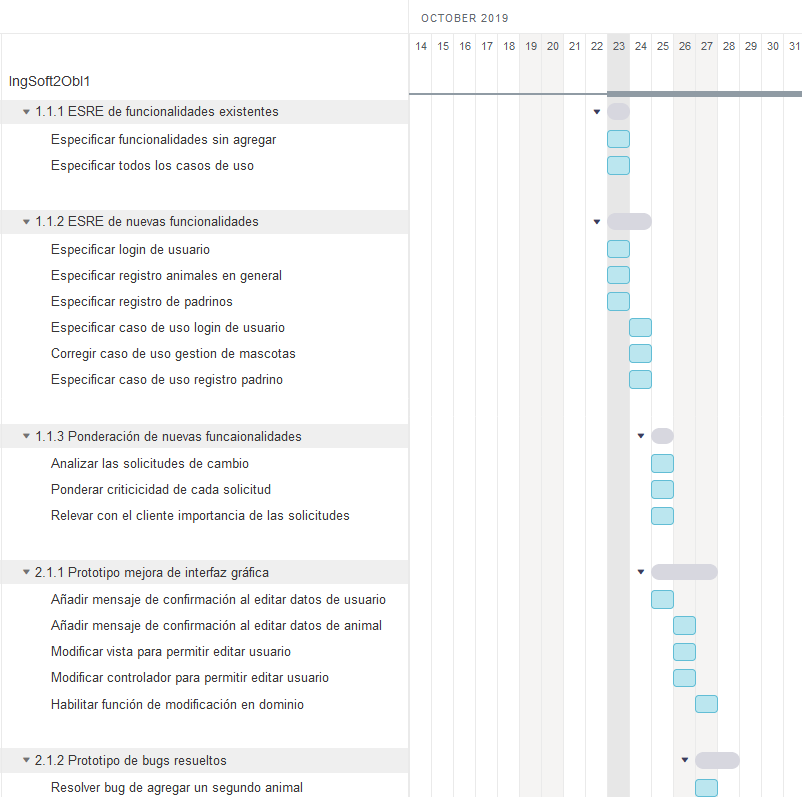
\includegraphics[scale=0.5]{Files/gannt1.png}
    \caption{Cronograma de tareas 1 de 3}
    \label{fig:clases}
\end{figure}


\begin{figure}[H]
    \centering
    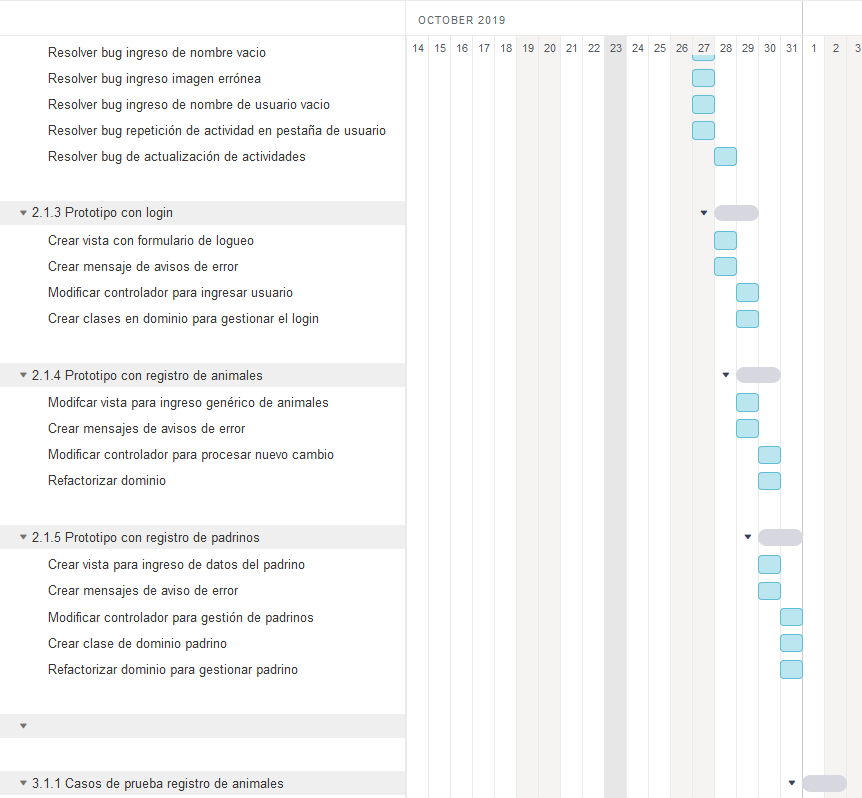
\includegraphics[scale=0.5]{Files/gannt2.png}
    \caption{Cronograma de tareas 2 de 3}
    \label{fig:clases}
\end{figure}


\begin{figure}[H]
    \centering
    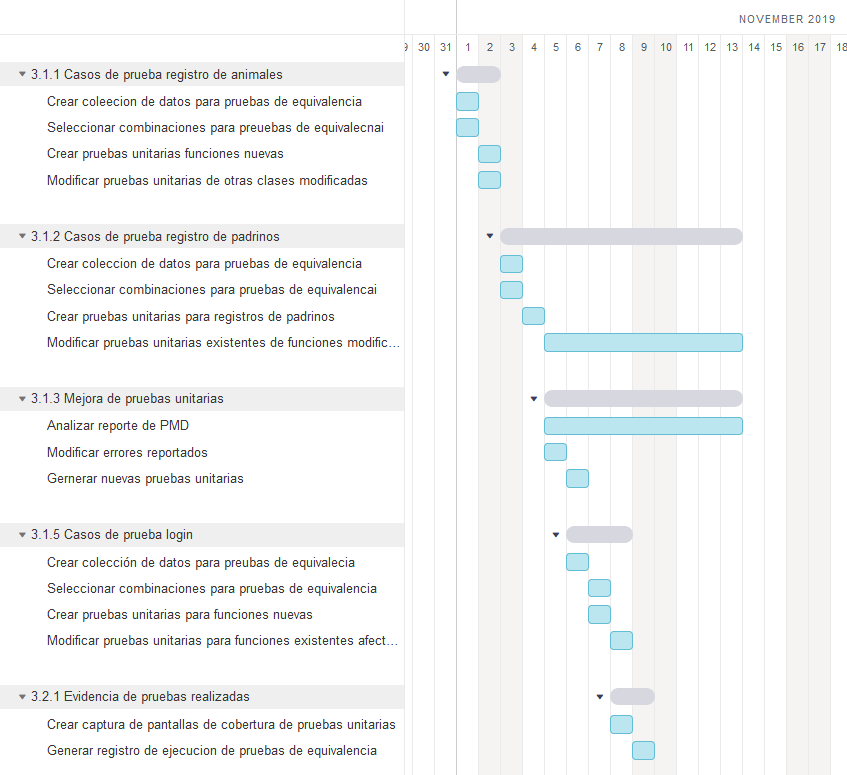
\includegraphics[scale=0.5]{Files/gannt3.png}
    \caption{Cronograma de tareas 3 de 3}
    \label{fig:clases}
\end{figure}
